\section{Einleitung}

Diese Ausarbeitung ist neben dem produzierten Quellcode das Resultat des
Master Informatik Teamprojekts von \autor im Sommersemester 2013 bis
Wintersemester 2013/2014.

Es geht darum den visuellen Editor der durch Spray generiert wird
von Eclipse Graphiti ins Web zu bringen, also mit den Webtechnologien
HTML, CSS, JavaScript und einer Webservertechnologie.
Spray soll also später in der Lage sein, auch genau diesen Spray
Web Editor zu generieren (parallel zu dem gewöhnlichen Graphiti Editor).

\subsection{Einführung in Spray}

\begin{quote}
The Graphiti framework is a new approach to create highly sophisticated
visual editors on top of the GEF framework.
Graphiti can easily be integrated with EMF as the
domain modeling framework. [...]
Spray aims to provide Domain Specific Languages (DSL) [...]
to describe Visual DSL Editors [...]
and provide code generation [...] to create the boilerplate code
for [...] the Graphiti framework. [...]
With the help of the tools created with Spray,
Graphiti based diagram editors can be created much faster
and reliable than doing it purely by hand. \citep{sprayWebpage}
\end{quote}

\noindent Das bedeutet: Spray bietet domänenspezifische Sprachen (DSLs) an,
um einen grafischen Editor zu beschreiben. Man könnte sagen, dass
man mit Spray eine Grammatik für grafische Editoren an die Hand bekommt.
Man beschreibt textuell das Layout und Aussehen von Shapes, und beschreibt
zudem was zulässige Verbindungen zwischen den einzelnen Shapes sind.
Resultat ist ein domänenspezifischer grafischer Editor.
Auf Abbildung \ref{fig.sprayArchi} ist der prinzipelle Spray zu Editor Ablauf. 

\begin{figure}[h!]
  \centering
  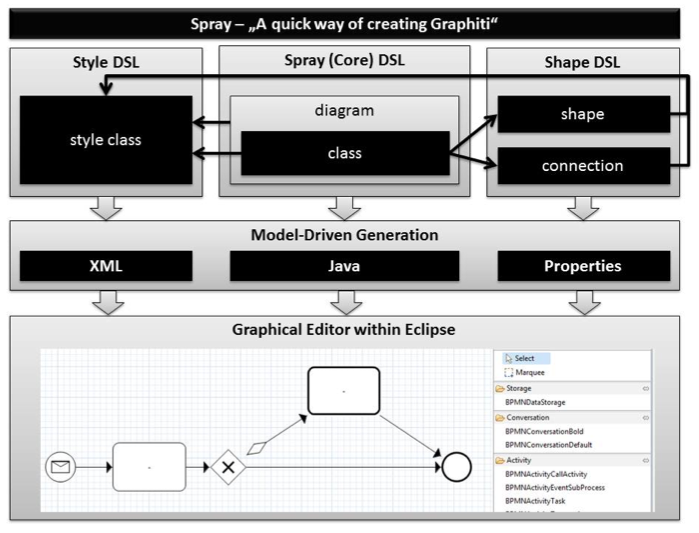
\includegraphics[width=1.0\textwidth]{Figures/SprayArchitektur.png}
  \caption{Prinzipelle Architektur von Spray. \citep[aus][S.~3]{sprayPaper}}\label{fig.sprayArchi}
\end{figure}

\subsection{Ziel von „Spray Web“}

Das hier Forschungsarbeit: „Wie könnte man die Sache prinzipiell angehen?“

\subsection{Ecore Metamodell}

\subsection{Graphiti}


\section{Anforderungen}

\subsection{Primitive Shapes}

\subsection{Connections}

\subsection{Compartments}

\subsection{Generalisierbarkeit}


\section{Architektur}


\section{Umsetzung}


\subsection{Shapes zeichnen}

\subsubsection{Toolkits}

\subsubsection{\dd}

\citep{dd}

\subsubsection{Shape Factory}

Rekursives Zeichnen der Shapes aus einer Definition

\subsubsection{Compartments}


\subsection{Code-Generierung}

\subsubsection{Shape Definitionen}

\subsubsection{Definitionen für ein zulässiges Modell}


\subsection{Validierung und Persistierung}

\subsubsection{Anwendung der abgeleiteten Modell Regeln}

Regeln abgeleitet aus dem Modell mit \dd abfangen.

\subsubsection{EMF REST}

\subsubsection{Ecore.js}

\subsubsection{Ecore mit Server}


\section{Nächste Ausbaustufen}

\subsection{Alternative Zeichentoolkits}

go.js oder digaram.js sind eleganter?
Unsere bisherigen Erkenntnisse einbringen.

\subsection{Pflege Codebasis}

Bisheriges verbessern, stabilisieren und testen.

\subsection{Kollobarationsfähigkeit}

\subsection{Validierung ausbauen}

Gibt es andere Möglichkeiten zu validieren oder zu persistieren?
Reine Client-Validierung, also Standalone im Browser oder doch Server?

\subsection{Spray Integration}

Den bisherigen Code in Spray vernünftige integrieren, mit Tests, sowie
den Dev und User Guide entsprechend erweitern.
Generator der Spray Grammatik übersetzt auf die neue Grammatik von Thomas u.a.
portieren?


\section{Zusammenfassung}

Fazi und Zusammenfassung der Ergebnisse.
